Description of the problem ($\FP+\CC+\MA+\BW$).

\subsection{Dynamic programming on trees}

Intro to dynamic programming on trees with subtree decomposition.
Introduce binarization as way of dealing with trees of larger arity.
Mention correctness requirements: substructure optimality and
overlapping subproblems.

\subsection{Introduction to our algorithm}

\maciek{We will want to go through all VM placements, for each of those do greedy matching and choose the cheapest.}

\maciek{Solution for subtree - how it can look like? It is ``partial matching''. Some matched VMs and chunks, but also some chunks transported out of subtree or some VMs/slots that will have chunks transported into from outside. So we charge already those incomplete matchings.}


Let's start by transforming our tree to binary tree with arbitrary
depth. We also introduce weights on edges (either $0$ or $1$). The
strategy we use is to clone every vertex $|children(v)| - 2$ times,
placing subsequent clones as right son of the previous one and placing
subsequent children as left son of the clone. Last child is placed as
right son of last clone.

Let's begin designing our algorithm by writing recursive formula for
minimal cost inclined by placing virtual machines in leaves of a given
tree. Our approach is to evaluate this function using bottom-up
technique using auxilary array, which yields a dynamic programming
solution. To find actual placements of virtual machines in addition to
the cost, we traverse the array backwards, following the path of
minimas.

Keep in mind that number of virtual machines is equal to number of
chunks. However, our function $f$ will be defined by structural
induction on the tree and we will invalidate the property of having
the same number of chunks and virtual machines in a given subtree
(which is true when we look at whole tree).

Let's define $f$ in following way. First argument is a subtree (with
available informations like number of chunks in its leaves), and the
second argument is number of virtual machines that we decided to place
in the subtree (given as first parameter). To calculate optimum
placement of $x$ virtual machines in subtree $T$ ($f(T, x)$) we will
consider every possible split of number $x$ into two positive integer
values: $l$ and $r = x - l$. We will place $l$ virtual machines in
left subtree of $T$ and $r$ virtual machines in right subtree of
$T$. Having such information allow us to compute how much cost we
incline through edge $e_1$ (which connects left subtree of $T$ to root
of $T$) and edge $e_2$ (which connects right subtree of $T$ to root of
$T$). In a given recursive call we charge only those two edges, rest
of edges will be charged is subsequent calls.

Our cost function consists of two factors. First one, communication
cost between virtual machines is easy to compute. We know how many
virtual machines are in left subtree, how many are in right subtree
and how many are in whole tree outside of $T$. For each pair of
virtual machines, first of which is in left subtree and second of
which is in right subtree, we charge $b_2 \cdot (w(e_1) +
w(e_2))$. For each pair of virtual machines, first of which is in left
subtree and second of which is outside $T$, we charge $b_2 \cdot
w(e_1)$. Right subtree case is symmetrical. Second factor of our cost
function is the cost of transferring chunks to virtual machines. Let's
call number of chunks in left subtree as $c_l$ and number of chunks in
right subtree as $c_r$. To incline minimal cost we connect chunks in
given subtree to virtual machines in the same subtree. If we can no
longer do that, because $v_i < c_i (i \in \{l,r\})$, then we connect
leftover chunks to virtual machines in second subtree of $T$. If we
can no longer do that, we connect leftover chunks outside of $T$. This
strategy is optimal, because connecting any other way can be amended
(TODO: need better argument here), inclining lower cost. Connections
inside either left or right subtrees inclines cost $0$ to edges $e_1$
and $e_2$. Connections between left and right subtree incline cost
$b_1
\cdot (w(e_1) + w(e_2))$. Connections from either subtree to outside
of $T$ inclines either $b_1 \cdot w(e_1)$ or $b_2 \cdot
w(e_2)$. Finally, we can write down our formula for $f$:

\begin{multline}
f(T, x) = min_{l \in \{0, \ldots, x\}} \{ f(T_l, l) + f(T_r, x - l) \\
+ TransferCost(T_l,l,T_r,x-l) \\ + ConnectionCost(l,x-l)\}
\end{multline}

One simplifying observation is that to calculate $TransferCost$ we can
just use the absolute value of difference between number of chunks and
number of virtual machines in a given subtree, without knowing which
is bigger, because in our model if there are some virtual machines
left, we know that some chunks from outside will use the same transfer
as if we have excessive chunks in the subtree.

\subsection{Algorithm}
\newcommand{\SumIndex}{\ensuremath{n}}
\begin{algorithm}[tbhp]
\DontPrintSemicolon % Some LaTeX compilers require you to use
%%\dontprintsemicolon instead
\SetAlgoNoEnd
\KwIn{$\Opt_{\SubstrateNode_l} , 
\Opt_{\SubstrateNode_r}, 
\ChunkCount_{\SubstrateNode_l},\ChunkCount_{\SubstrateNode_r} $}
$\ChunkCount_\SubstrateNode = \ChunkCount_{\SubstrateNode_l} +
\ChunkCount_{\SubstrateNode_r}$\;
\For{$\SumIndex \in \{0,\dots,\Vms\}$}{
  \For{$i \in \{0,\dots,\SumIndex\}$}{ \If{$\Opt_\SubstrateNode[\SumIndex]
  > \Opt_{\SubstrateNode_l}[i] +
\Opt_{\SubstrateNode_r}[\SumIndex - i]$}{
	$\Opt_\SubstrateNode[\SumIndex] \gets \Opt_{\SubstrateNode_l}[i]
	+
\Opt_{\SubstrateNode_r}[\SumIndex - i]$\;
    } }
  
 $bw \gets (\Vms -
\SumIndex) \cdot \SumIndex \cdot \CostCom +   |i - 
\ChunkCount_\SubstrateNode| \cdot \CostTrans$\; 
  \eIf{$bw \leq \Capacity(\Uplink(v))$}{
    $\Opt_\SubstrateNode[\SumIndex] \gets \Opt_\SubstrateNode[\SumIndex]
    + bw$\; }{ $\Opt_\SubstrateNode[\SumIndex] \gets \infty$\; } }
%
\caption{$aggregate(\SubstrateNode \in \SubstrateNodes)$}
\label{algo:dynAggregation}
\end{algorithm}

List all needed functions like distance, counter of number of chunks
in subtree.

Tell how to go back through the array to reconstruct the actual
placements. Following path of minimas. Other approach is to store pointers to minimas on lower levels as those are chosen.

(Base case) We fill the entire array $Opt_l$ for the leaf $l$ with zeros. It means that we allow hosting $0, 1, \ldots, n$ VMs in this leaf. We can restrict the number of VMs that are hosted in the same leaf by some constant $x$ (that can be independent for every leaf) by setting $Opt_l[x+1] = Opt_l[x+2] = \ldots = Opt_l[n] = \infty$.

\subsection{Algorithm correctness}

\subsubsection{Bandwidth correctness.}

\begin{lemma}
Let's say that we calculated solution for our instance of VC with
ignoring the bandwidth. Then we analyzed every link and it turned out
that some of them exceed their capacity. Then the instance is
infeasible and we cannot fix that by choosing any other matching (even
suboptimal one).
\end{lemma}

It might happen that this lemma does not hold, beware!

\maciek{Below there is emergency lemma in case that above lemma does not hold. In case above lemma is true it implies that below lemma is true.}
\begin{lemma}
An instance of $\Problem$ is infeasible iff. algorithm returns
$\infty$.
\end{lemma}
\begin{proof}
  ($\rightarrow$)

  ($\leftarrow$) \end{proof}

\maciek{I think that we do not need that lemma, it might be obvious. I leave it there just in case.}
\begin{lemma}
  If algorithm returns solution $\Sol$ of cost $\neq \infty$, then in
  $\Sol$ no link exceeds its capacity limit.  \end{lemma}

\subsubsection{Substructure optimality without bandwidth.}

Definition of partial matching (matching + transporting imbalanced
chunks out of tree and transporting chunk into imbalanced VMs from
outside the tree). Definition of partial matching optimality
(parametrized by number of VMs, subtree and chunks; best among all
possible that match the same chunks and transports the imbalance).
\begin{lemma}

Let's consider an arbitrary tree $T$ with chunks $c_i$ and number of
VMs $v$. Than $f(T, v)$ is cost of optimal partial matching.

\end{lemma}

\begin{proof}
Proof by structural induction. First, we take definition of $f$, which
contains values of $f$ for left and right subtree for different number
of VMs (but which sum to $v$). We can assume by induction that those
are optimal. Then we calculate the cost of communication and matching
between left and right subtree (also in $f$'s definition. Then we
choose the minimum cost one. We argue that this one is optimal partial
matching, and we use optimality of greedy matching for that.

Also, we use the uplink lemma to show that choosing optimal partial
matching in left and right subtree does not generate excessive
bandwidth on both uplink edges (we might have doubted that because
optimal partial matchings were restricted to their subtrees and we
might thought that there is some other more costly matching that has
less bandwidth on uplink - to save there).

Also, we use optimality of greedy matching that is in matching
chapter.
\end{proof}

\subsubsection{Substructure optimality with bandwidth.}
\begin{lemma}
Function $f$ modified to take bandwidth into account returns cost of feasible optimal partial matching (or no feasible solution exists).
\end{lemma}

\begin{proof}

For a given positions of VMs if optimal matching is infeasible, no other (even suboptimal) matching is feasible. Our algorithm checks every possible placement of VMs, so if there would be any feasible placement, our algorithm would have found feasible matching for that (the optimal one).

\end{proof}
\subsection{Running time and memory consumption analysis}

We spend certain amount of time in every of $2|T|$ vertices of binary
tree (factor 2 is inclined there because of binary
transformation). This time can be bound by iterating over splits of
$n$ into two integers, times some constant and we do it for every
possible number of VMs from $0$ to $n$. Therefore, resulting running
time is $O(Nn^2)$.

\begin{figure}
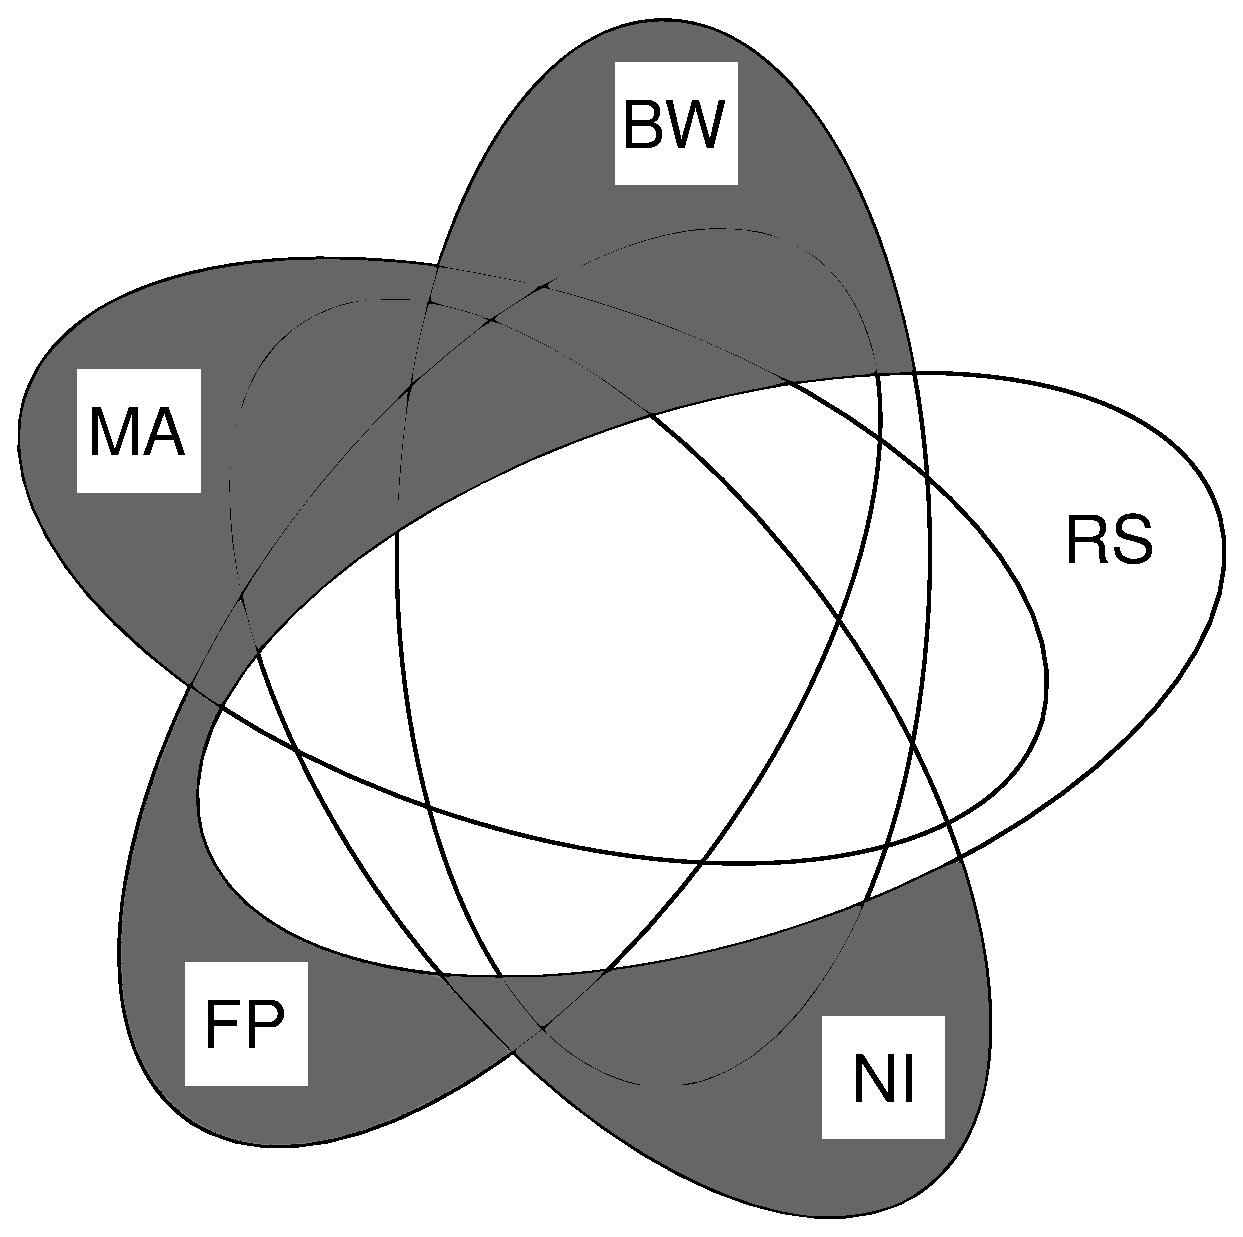
\includegraphics[width=\columnwidth]{figs/venn_dp.pdf}
\caption{Property combinations which can be solved by our dynamic prorgramming 
appraoch.}
\label{fig:venn_dp}
\end{figure}

\carlo{Figure~\ref{fig:venn_dp} shows illustrates which problem 
combiantions can be solved by the presented dynamic programming
approach.}
